\documentclass[a4paper,10pt,english]{article}
\usepackage[utf8]{inputenc}
%\bibliography{references.bib}
% Standard stuff
\usepackage{amsmath,amssymb,graphicx,babel,varioref,verbatim,amsfonts,float}
\usepackage[a4paper, total={6in, 8in}]{geometry}
%\usepackage{biblatex}
\graphicspath{{C:/Users/elini/Documents/FYS-STK4155/FYS-STK4155/project1/report/figures/}}%{C:/Users/elini/Documents/Master/mastermal-ita}

\usepackage{csquotes}
\usepackage[round]{natbib}
\bibliographystyle{plainnat}
\usepackage[bottom]{footmisc}
\usepackage{multirow}
\usepackage{adjustbox}
\usepackage{tabularx}
\usepackage[font=small]{caption}
\usepackage{booktabs} %nicer tables
%\usepackage{subcaption}
\usepackage{bm}
\usepackage{booktabs} %nicer tables
\usepackage[font=small]{caption}
\usepackage{threeparttable}
% arrows upuparrows downuparrows
\newcommand{\updownarrows}{\uparrow\mathrel{\mspace{-1mu}}\downarrow}
\newcommand{\downuparrows}{\downarrow\mathrel{\mspace{-1mu}}\uparrow}
\renewcommand{\upuparrows}{\uparrow\uparrow}
\renewcommand{\downdownarrows}{\downarrow\downarrow}

\usepackage{mathrsfs} % fancy lettering
\newcolumntype{Y}{>{\centering\arraybackslash}X} % centered columns with textwidth
% colors in text
\usepackage[usenames,dvipsnames,svgnames,table]{xcolor}
% Hyper refs
\usepackage[colorlinks,linkcolor=black,citecolor=black]{hyperref}

% Document formatting
\setlength{\parindent}{2em}
\setlength{\parskip}{1.5mm}

\def\code#1{\texttt{#1}} % make single word look like code, comand \code{...}
%Equation formatting
\usepackage{physics}	% For derivative fraction symbol, partial and total
\newcommand\numberthis{\addtocounter{equation}{1}\tag{\theequation}} % number certain equations in align*
\newcommand{\matr}[1]{\mathbf{#1}}	% Thick line for matriced and vectors in mathmode

%Color scheme for listings
\usepackage{textcomp}
\definecolor{listinggray}{gray}{0.9}
\definecolor{lbcolor}{rgb}{0.9,0.9,0.9}

%Listings configuration
\usepackage{listings}
\lstset{
	backgroundcolor=\color{lbcolor},
	tabsize=4,
	rulecolor=,
	language=python,
        basicstyle=\scriptsize,
        upquote=true,
        aboveskip={1.5\baselineskip},
        columns=fixed,
	numbers=left,
        showstringspaces=false,
        extendedchars=true,
        breaklines=true,
        prebreak = \raisebox{0ex}[0ex][0ex]{\ensuremath{\hookleftarrow}},
        frame=single,
        showtabs=false,
        showspaces=false,
        showstringspaces=false,
        identifierstyle=\ttfamily,
        keywordstyle=\color[rgb]{0,0,1},
        commentstyle=\color[rgb]{0.133,0.545,0.133},
        stringstyle=\color[rgb]{0.627,0.126,0.941}
        }
        
\newcounter{subproject}
\renewcommand{\thesubproject}{\alph{subproject}}
\newenvironment{subproj}{
\begin{description}
\item[\refstepcounter{subproject}(\thesubproject)]
}{\end{description}}

%Lettering instead of numbering in different layers
%\renewcommand{\labelenumi}{\alph{enumi}}
%\renewcommand{\thesubsection}{\alph{subsection}}

%opening
\title{Regression analysis and resampling methods}
\author{Elisabeth Strøm}

\begin{document}

\maketitle

\pagebreak

\tableofcontents

\pagebreak


\section{Introduction}
In this project we test three different linear regression methods: The Ordinary Least Squares (OLS), Ridge regression, and Lasso regression.

This project consists of two parts.
First, we try to estimate the Franke function \citep{Franke}, having created a noisy dataset from the function. This is to see how well our algorithm works. We also implement $k$-fold cross validation.

Next, we sample data taken of the terrain, from somewhere in the world (SOURCE), and try to recreate it by using our regression models.

In Section \ref{sec:method}, we go through the theory behind the methods we will use, and also show how we will implement them numerically.

Our results can be seen in Section \ref{sec:results}, and we will discuss them in Section \ref{sec:discussion}. Finally, we sum up our conclusions in Section \ref{sec:conclussion}.

%%%%%%%%%%%%%%%%%%%%%%%%%%%%%%%%%%%%%%%%%%%%%%%%%%%%%%%%%%%
%
%                            METHOD
%
%%%%%%%%%%%%%%%%%%%%%%%%%%%%%%%%%%%%%%%%%%%%%%%%%%%%%%%%%%
\section{Method}\label{sec:method}
Here we go through our methods of linear regression, while in \ref{sec:implementation}, we show how we implement them numerically.

Say we have a dataset consisting of $\{y_i, \bm{{x}}_i, i=0...n-1\}$, where $y_i=y(\bm{{x}}_i)$ is the outcome, or the response, and $\bm{{x}}_i$ is the predictor, or independent variable.
The idea behind linear regression, is determine the true function, $f(\bm{{x}})$, from our noisy data 
\begin{equation}
y(\bm{{x}}_i)=f(\bm{{x}}_i) + \epsilon_i.
\end{equation}
Here, $\bm{{\epsilon}}$ is the noise which we assume to be normally distributed with mean $\mu=0$ and standard deviation $\sigma$, $\mathcal{N}(\mu,\sigma^2)=\frac{1}{\sqrt{2 \pi \sigma^{2}}} e^{-(x-\mu)^{2} / 2 \sigma^{2}}$.

Through a regression analysis, we estimate $f$ by the function $\bm{{\tilde y}}$. For one predictor $\bm{{x}}$ this can be written as
\begin{equation}
y_i \approx \tilde y_i + \epsilon_i = \sum_{j=0}^{m-1}\beta_j \bm{{x}}_{i,j} + \epsilon_i.
\end{equation}
Here $\beta_j$ are called the regression coefficients, and $x_{i,j}$ are the terms in the function $\tilde y_i$.

In matrix notation,
\begin{equation}\label{eq:y_tilde}
\bm{{\tilde y}} = \bm{{X}}\bm{{\beta}},
\end{equation}
where $\bm{{y}}=[y_0, y_1, \dots, y_{n-1}]^{T}$, $\bm{{\beta}}=[\beta_0, \beta_1, \dots, \beta_{n-1}]^{T}$, and $\bm{{X}}$ is the design matrix,
\begin{equation}\label{eq:design_matrix}
\bm{{X}}=
\begin{bmatrix}
x_{00} & x_{01} & \dots   & x_{0,m-1} \\
x_{10} & x_{11} & \dots   & x_{1,m-1} \\
\vdots & \vdots & \ddots  & \vdots \\
x_{n-1,0} & x_{n-1,1} & \dots   & x_{n-1,m-1}
\end{bmatrix},
\end{equation}

The $\beta$-coefficients, are found by optimizing the the Mean Squared Error,
\begin{equation}
MSE(\bm{{y}},\bm{{\tilde y}}) = \frac{1}{n}\sum^{n-1}_{i=0}(y_i-\tilde y_i)^{1/2},
\end{equation}
via the cost function
\begin{equation}
C(\bm{{X}},\bm{{\beta}}) = \frac{1}{n}\sum^{n-1}_{i=0}(y_i-\tilde y_i)^{1/2} = \mathrm{E}[(\bm{{y}}-\bm{{\tilde y}})^2].
\end{equation}

We will also look at the $R^2$ score function, defined as
\begin{equation}
R^2(\bm{{y}},\bm{{\tilde y}})= 1 - \frac{\sum_{i=0}^{n-1}(y_i-\tilde y_i)^2}{\sum_{i=0}^{n-1}(y_i- \bar y)^2},
\end{equation}
where $\bar y$ is the mean value, $\frac{1}{n}\sum^{n-1}_{i=0}y_i$. Then the closer $R^2$ is to 1, the better is our fit.

The confidence interval of a parameter $X$ at 95\% confidence, assuming a Gaussian distribution, is defined as
\begin{equation}
CI_{X}^{0.95} = \mathrm{E}[X] \pm 1.96\cdot \mathrm{STD}[X],
\end{equation}
where $\mathrm{E}(X)$ is the mean of $X$, and $\mathrm{STD}[X]$ is the standard deviation of $X$.

For the $\beta$-parameters this becomes,
\begin{equation}
CI_\beta-j= \beta_j \pm 1.96\sqrt{\mathrm{Var}(\beta_j)}.
\end{equation}

We aim to find $\tilde y_i$, through three different methods: The Ordinary Least Square (OLS), Ridge regression, and Lasso regression, which are outlined in the next three subsections.


\subsubsection{Decomposing the cost function}

The cost function can be decomposed into three terms, the bias squared of $\bm{{\tilde y}}$, the variance of $\bm{{\tilde y}}$, and the irreducible error variance, which is just $\mathrm{Var}(\epsilon_i)=\sigma^2$,

\begin{align*}
\mathrm{{E}}[\bm{{y}}-\bm{{\tilde y}}] &= \mathrm{{E}}[(\bm{{f}} + \bm{{\epsilon}} - \bm{{\tilde y}})^2]\\
	&= \mathrm{{E}}[(\bm{{f}}+\bm{{\epsilon}} - \bm{{\tilde y}} + \mathrm{{E}}[\bm{{\tilde y}}] - \mathrm{{E}}[\bm{{\tilde y}}])]\\
	&= \mathrm{{E}}[(\bm{{f}} - \mathrm{{E}}[\bm{{\tilde y}}])^2] + \mathrm{{E}}[\bm{{\epsilon}}^2] + \mathrm{{E}}[(\mathrm{{E}}[\bm{{\tilde y}}]-\bm{{\tilde y}})^2]\\
	 &\hspace{1em} + 2\mathrm{{E}}[\bm{{\epsilon}}(\bm{{f}}-\mathrm{{E}}[\bm{{\tilde y}}])] + 2\mathrm{{E}}[(\bm{{f}} - \mathrm{{E}}[\bm{{\tilde y}}])(\mathrm{{E}}[\bm{{\tilde y}}]-\bm{{\tilde y}})] + 2\mathrm{{E}}[\bm{{\epsilon}}(\mathrm{{E}}[\bm{{\tilde y}}]- \bm{{\tilde y}})]\\
	 &= (\bm{{f}} - \mathrm{{E}}[\bm{{\tilde y}}])^2 + \sigma^2 + (\mathrm{{E}}[\bm{{\tilde y}}]-\bm{{\tilde y}})^2\\
	 &= \mathrm{Bias}^2(\bm{{\tilde y}}) + \mathrm{Var}(\bm{{\tilde y}}) + \sigma^2,
\end{align*}
where in the last term, $\mathrm{Bias}^2(\bm{{\tilde y}}) = (\bm{{f}} - \mathrm{{E}}[\bm{{\tilde y}}])^2$, and $\mathrm{Var}(\bm{{\tilde y}}) = (\mathrm{{E}}[\bm{{\tilde y}}]-\bm{{\tilde y}})^2$.

The cross terms in the fourth line above, disappears as follows,
\begin{align*}
2\mathrm{{E}}[\bm{{\epsilon}}(\bm{{f}}-\mathrm{{E}}[\bm{{\tilde y}}])] &= 2\mathrm{{E}}[\bm{{\epsilon}}]\mathrm{{E}}[\bm{{f}}-\mathrm{{E}}[\bm{{\tilde y}}]] = 0,\\
2\mathrm{{E}}[\bm{{\epsilon}}(\mathrm{{E}}[\bm{{\tilde y}}]- \bm{{\tilde y}})] &= 2\mathrm{{E}}[\bm{{\epsilon}}]\mathrm{{E}}[(\mathrm{{E}}[\bm{{\tilde y}}]- \bm{{\tilde y}})] = 0
\end{align*}
where we have used that the expectation value, or the mean of the noise term $\bm{{\bm{{\epsilon}}}}$ is 0,
\begin{align*}
2\mathrm{{E}}[(\bm{{f}} - \mathrm{{E}}[\bm{{\tilde y}}])(\mathrm{{E}}[\bm{{\tilde y}}]-\bm{{\tilde y}})] &= 2\mathrm{{E}}[\bm{{f}} - \mathrm{{E}}[\bm{{\tilde y}}]]\mathrm{{E}}[(\mathrm{{E}}[\bm{{\tilde y}}]-\bm{{\tilde y}})]\\
	&= 2(\bm{{f}} - \mathrm{{E}}[\bm{{\tilde y}}])(\mathrm{{E}}[\bm{{\tilde y}}]-\mathrm{{E}}[\bm{{\tilde y}}])\\
	&= 2(\bm{{f}} - \mathrm{{E}}[\bm{{\tilde y}}])\cdot 0\\
	& = 0.
\end{align*}

Generally, as the complexity of our model increases, for instance the polynomial degree where we to fit a polynomial to our data, the bias will decrease, while the variance increases.

A simpler model is easier to train, but have a lower predictive power on more complex problems. A complex model may fit the data better, but will also be prone to overfitting as the complexity increases, sampling the noise instead of the true function $f$. This means that the variance of $\bm{{\tilde y}}$ estimated from different training set, will be high. Ideally we would have a low-variance and low-bias model, so we will have to balance the two factors. Linear regression is in general a low variance procedure. 

%%%%%%%%%%%%%%%%%%%%%%%%%%%%%%%%%%%%%%%%%%%%%%%%%%%%%%%%%%%
%
%                       OLS
%
%%%%%%%%%%%%%%%%%%%%%%%%%%%%%%%%%%%%%%%%%%%%%%%%%%%%%%%%%%
\subsection{Ordinary Least Squares regression}
We start with the simplest of the regression methods: The Ordinary Least Square.

The idea behind this method, is to fit a polynomial, $\bm{{\tilde y}}$, to our, usually, noisy data $\bm{{y}}$, and try to model the underlying, true function $f$. In the case of one predictor $\bm{{x}}$,
\begin{equation}
y_i \approx \tilde y_i + \epsilon_i = \sum_{j=0}^{m-1}\beta_j \bm{{x}}^{j}_i + \epsilon_i.
\end{equation}
So the elements of the design matrix $\bm{{X}}$ (Equation \ref{eq:design_matrix})
are now $x_{i,j}=x_i^j$.

In our project, we try to recreate the Franke function, which has two independent parameters, $x, y \in [0, 1]$,
\begin{equation}
\begin{aligned} 
f(x, y) &=\frac{3}{4} \exp \left(-\frac{(9 x-2)^{2}}{4}-\frac{(9 y-2)^{2}}{4}\right)+\frac{3}{4} \exp \left(-\frac{(9 x+1)^{2}}{49}-\frac{(9 y+1)}{10}\right) \\
&+\frac{1}{2} \exp \left(-\frac{(9 x-7)^{2}}{4}-\frac{(9 y-3)^{2}}{4}\right)-\frac{1}{5} \exp \left(-(9 x-4)^{2}-(9 y-7)^{2}\right).
\end{aligned}
\end{equation}

Our estimate of $f(\bm{{x}},\bm{{y}})$, is denoted as $\bm{{\tilde z}}$, and our noisy data we perform an analysis on, is then $z_i= f(\bm{{x}}_i,\bm{{y}}_i) + \epsilon_i$, where $\epsilon_i\sim \mathcal{N}(0,1)$. The elements of the design matrix will then also assume a slightly different shape, where the order of the polynomial $\tilde z_i$ is a result of the polynomial order of both $\bm{{x}}_i$ and $\bm{{y}}_i$ multiplied together. We will get back to how to implement this in Section \ref{sec:implementation}.

The $\bm{{\beta}}$ coefficients are calculated from
\begin{equation}
\bm{{\beta}}^\mathrm{OLS} = (\bm{{X}}^T\bm{{X}})^{-1}\bm{{X}}^T\bm{{z}},
\end{equation}
for the $\bm{{\tilde z}}$, calculated from $\bm{{X}}$ (Equation \ref{eq:y_tilde}) for different polynomial orders, that minimizes the Mean Squared Error, or the predictive error.

The variance of $\bm{{\beta}}$ is,
\begin{equation}
\mathrm{Var}(\bm{{\beta}}) = \sigma^2\cdot\mathrm{diag}(\bm{{X}}^T\bm{{X}}^{-1}),
\end{equation}
where $\sigma^2$ is still the variance of the noise $\bm{\epsilon}$.
%%%%%%%%%%%%%%%%%%%%%%%%%%%%%%%%%%%%%%%%%%%%%%%%%%%%%%%%%%%
%
%                       Ridge
%
%%%%%%%%%%%%%%%%%%%%%%%%%%%%%%%%%%%%%%%%%%%%%%,%%%%%%%%%%%%
\subsection{Ridge and Lasso regression}
In our Ridge and Lasso regression analyses, we still aim to fit a polynomial to $f$, but now with a penalty parameter, $\lambda$. $\lambda$ will minimize the $\beta$ parameters.

The $\beta$ parameters for our Ridge analysis, is calculated from
\begin{equation}
\bm{{\beta}}^\mathrm{Ridge} = (\bm{{X}}^T\bm{{X}} + \lambda \bm{{I}})^{-1}\bm{{X}}^T\bm{{z}},
\end{equation}
where $\bm{{I}}$ is the identity matrix, $\bm{{I}} = \mathrm{diag}(1,1,\dots , 1)$ of the same shape as $\bm{{X}}^T\bm{{X}}$, that is, $n\times n$.

The variance of $\bm{{\beta}}^\mathrm{Ridge}$ is,
\begin{equation}
\mathrm{Var}(\bm{{\beta}}^\mathrm{Ridge}) = \sigma^2\cdot\mathrm{diag}([\bm{{X}}^T\bm{{X} + \lambda \bm{I}}]^{-1}\bm{{X}}^T\bm{{X}}\{[\bm{{X}}^T\bm{{X} + \lambda \bm{I}}]^{-1}\}^T),
\end{equation}

In our Lasso analysis, we do not have an analytical expression for the $\beta$ coefficients, but they will instead be found by using \code{sklearn}'s \code{Lasso} function.

The variance of $\bm{\beta}^\mathrm{Lasso}$ is found by minimizing the Lasso cost function $k=5$ times through $k$-fold cross-validation using \code{sklearn}, and then finding the variance of the $k$ $\bm{\beta}^\mathrm{Lasso}$ that are found.% The 95\% confidence interval is in this case, $\bar{\bm{{\beta}}}^\mathrm{Lasso} \pm 1.96\cdot\mathrm{STD}(\bm{\beta})\/\sqrt{k-1}$
 
%%%%%%%%%%%%%%%%%%%%%%%%%%%%%%%%%%%%%%%%%%%%%%%%%%%%%%%%%%%
%
%                     IMPLEMENTATION
%
%%%%%%%%%%%%%%%%%%%%%%%%%%%%%%%%%%%%%%%%%%%%%%%%%%%%%%%%%%
\subsection{Implementation}\label{sec:implementation}
Here we go through how we implemented our regression analyses.

The first thing we do is create the $\bm{x}$ and $\bm{y}$. We make two arrays with evenly spaced points, for a total of a 100 each, between 0 and 1. Then we use the \code{numpy} command \code{meshgrid(x,y)} to create a meshgrid. $\bm{x}$ and $\bm{y}$ are then used to construct the Franke function $\bm{z}=f(\bm{x}, \bm{y})$. Next we flatten the arrays, and copy $\bm{z}$ and add the normally distributed noise $\bm{\epsilon}$. We know have the true function, \code{z1\_true} and the noisy function \code{z1\_noise},
\begin{verbatim}
z = FrankeFunction(x, y)
z1_true = np.ravel(z)
# adding noise
z1_noise = np.ravel(z) + np.random.normal(0, stddev, size=z1_true.shape) 
\end{verbatim}

Next thing to do is create the design matrix $\bm{X}$. It is made so that the polynomial degree increases with the columns. Say we have a 2nd order polynomial, the first row then looks like
\begin{equation*}
x_{0,*} = [1, x_0, y_0, x_0^2, x_0y_0, y_0^2].
\end{equation*} 

To calculate $\bm{{\beta}}$ for OLS and Ridge regression, we need to be able to invert $\bm{X}^T\bm{X}$. We do this through a singular value decomposition
\begin{verbatim}
	U, s, Vt = np.linalg.svd(X)
	Sigma = np.zeros((len(U),len(Vt)))
	
	for i in range(0,len(Vt)):
		Sigma[i,i] = s[i]
	Sigma_inv = np.linalg.pinv(Sigma)
	X_inverted = np.matmul(Vt.T, np.matmul(Sigma_inv,U.T))
\end{verbatim}

Now, finding $\bm{{\tilde z}}$ is straight forward. Note that we will train our algorithm on the noisy data $\bm{z}^\mathrm{noise}$, but assert the fit by calculating MSE with the true Franke function $\bm{z}^\mathrm{true}$.

\subsubsection{$k$-fold Cross-Validation}
We implement the $k$-fold Cross-Validation. Here our data is shuffled and split into $k=5$ equal parts. $1/5$ is used as test data, wile the rest is training data. We then perform a regression analysis $k$ times, where we change which is the test set every time. For each analysis, we estimate the $\mathrm{MSE}$, and then, finally we take the mean of the $k$ error estimates. MSE is calculated both for the test, and training set.

\subsubsection{Standardizing the data}
We standardize the datasets in the following way: For the training set $\bm{X^\mathrm{train}}$,  we subtract the mean of each column from that column, and then we divide each column with the standard deviation of each column,
\begin{equation}
\bm{X}_{*,j}^\mathrm{train,c} = \frac{\bm{X}_{*,j}^\mathrm{train}-E[\bm{X}_{*,j}^\mathrm{train}]}{\mathrm{STD}(\bm{X}_{*,j}^\mathrm{train})}, \qquad\text{for } j=1,2,\dots, m-1.
\end{equation}
For $z$, we subtract the mean only, $\bm{z}^\mathrm{train,c}= \bm{z}^\mathrm{train,c}- \mathrm{E}[\bm{z}^\mathrm{train,c}]$

We apply these same transformations to the test set, that is,
\begin{equation}
\bm{X}_{*,j}^\mathrm{test,c} = \frac{\bm{X}_{*,j}^\mathrm{test}-E[\bm{X}_{*,j}^\mathrm{train}]}{\mathrm{STD}(\bm{X}_{*,j}^\mathrm{train})}, \qquad\text{for } j=1,2,\dots, m-1.
\end{equation}
and $\bm{z}^\mathrm{test,c}= \bm{z}^\mathrm{test,c}- \mathrm{E}[\bm{z}^\mathrm{train,c}]$. The columns now have a mean equal to 0, and a standard deviation equal to 1.

We add the mean again when calculating $\bm{{\tilde z}}$, that is
\begin{align}
\bm{\tilde z}^{train} &=\bm{z}^{train,c} + \mathrm{E}[\bm{z}^\mathrm{train,c}]\\
\bm{\tilde z}^{test} &=\bm{z}^{test,c} + \mathrm{E}[\bm{z}^\mathrm{train,c}].
\end{align}

Standardizing the data is not that important for the OLS method, but rather for Ridge and Lasso, where we have the penalty $\lambda$. $\lambda$ puts constraints on the $\beta$-coefficients, but the coefficients size depends on the magnitude of each variable.
It is therefore important to get the data on the same scales, so that no variable is punalized unfairly, and to be able to see which factors truly contribute the most to $\bm{\tilde z}$. Also, we no longer have an intercept, but it can be interpreted as being the $\mathrm{E}[\bm{z}^\mathrm{train,c}]$.

\subsubsection{Linear regression}
We first run the three regression analyses on the Franke Function data. Given that we know the true function already, we will train our algorithm with the noisy data, but calculate the MSE using the true function. 

Next we move onto the terrain data, where we used the files found together with the project instructions. This is a quite large dataset, so we chose a small cutout, just the first 1000 pixels in $x$ and $y$ direction. We down-sampled this image, by only including every 30th pixel in either direction.   

For the OLS, we calculate MSE for several polynomial degrees, to find which one offers the best fit.

For Ridge and Lasso, we must also find the best fit $\lambda$ parameter that together with the right polynomial, minimizes the MSE.

The result of our analyses can be found in Section \ref{sec:results}.
%%%%%%%%%%%%%%%%%%%%%%%%%%%%%%%%%%%%%%%%%%%%%%%%%%%%%%%%%%%
%
%                     RESULTS
%
%%%%%%%%%%%%%%%%%%%%%%%%%%%%%%%%%%%%%%%%%%%%%%%%%%%%%%%%%%
\section{Results}\label{sec:results}
Here we show the results of our regression analyses on the Franke function, and on the terrain data.

\subsection{The Franke function}
The best fit polynomial order, $\lambda$, the minimum predictive error MSE, and $R^2$ for each of the regression models, including cross-validation, can be found in Table \ref{tab:1}. This will be discussed at the end of this section, but first we will go through the intermediate results.

Having produced the true and noisy data as stated in Section \ref{sec:implementation}, we start by fitting a 5th order polynomial to \code{z1\_noise}. Unless stated otherwise, assume $\bm{X}$ is standardized, and $\bm{z}^{noise}$ is mean-centered.

For an Ordinary Least squares analysis, the $\beta$ parameters along with their confidence intervals at 95\%, can be seen in Figure \ref{fig:1}. We see that the confidence intervals are quite large in places, but we were not able to ascertain as to why.

\begin{figure}[H]
	\centering
	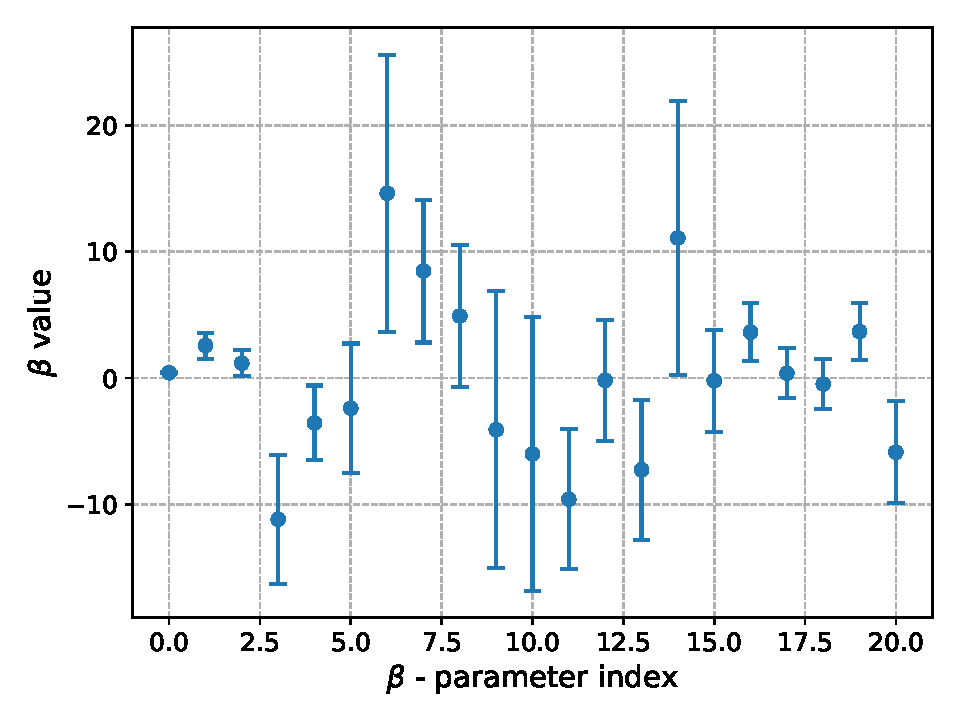
\includegraphics[scale=0.6]{a_CI_betaOLS_st_wb0.pdf}
\caption{The values of the parameters $\beta$ found from an Ordinary Least Squares regression analysis, are shown on the $y$-axis, while the index of the parameters are on the $x$-axis. The errorbars are calculated at 95\% confidence}
	\label{fig:1}
\end{figure}

Still, the MSE score is quite good, at $MSE(\bm{z}^\mathrm{true,test}, \bm{\tilde z})=4.09\cdot 10 ^{-3}$, and $R^2(\bm{z}^\mathrm{true,test}, \bm{\tilde z})=0.95$

Double checking our results against that found by \code{sklearn} using \code{LinearRegression}, showed that they were approximately the same.

\subsubsection{Cross-validating}
Next we used $k=5$-fold cross validation on our data.
We find now a very similar error as before, $MSE = 4.62\cdot 10^{-3}$, and $R^2= 0.94$.

Assuming we did not know the true underlying function, and we used our noisy model instead to calculate the error, we find
$MSE(\bm{z}^\mathrm{noise,test}, \bm{\tilde z}) = 1.19$,
which should be the irreducible error variance, that is, $\sigma^2$, which in our case we had chosen as 1, so this too is a good result.


\subsubsection{ Bias-Variance tradeoff}
We try to create a figure similar to Figure 2.11 of Hastie, Tibshirani, and Friedman, which shows the test and training error as a function of the complexity of the model. In our case, the complexity is the polynomial degree.

To reproduce this figure, we will pretend we do not know the true model, and use the noisy data alone. We then get the diagram in Figure \ref{fig:2}. Lowest MSE is still found at the 5th polynomial order, like before. Here we see that the test error reaches a minimum, but the training error continuously decreases.
 
 \begin{figure}[H]
 	\centering
 	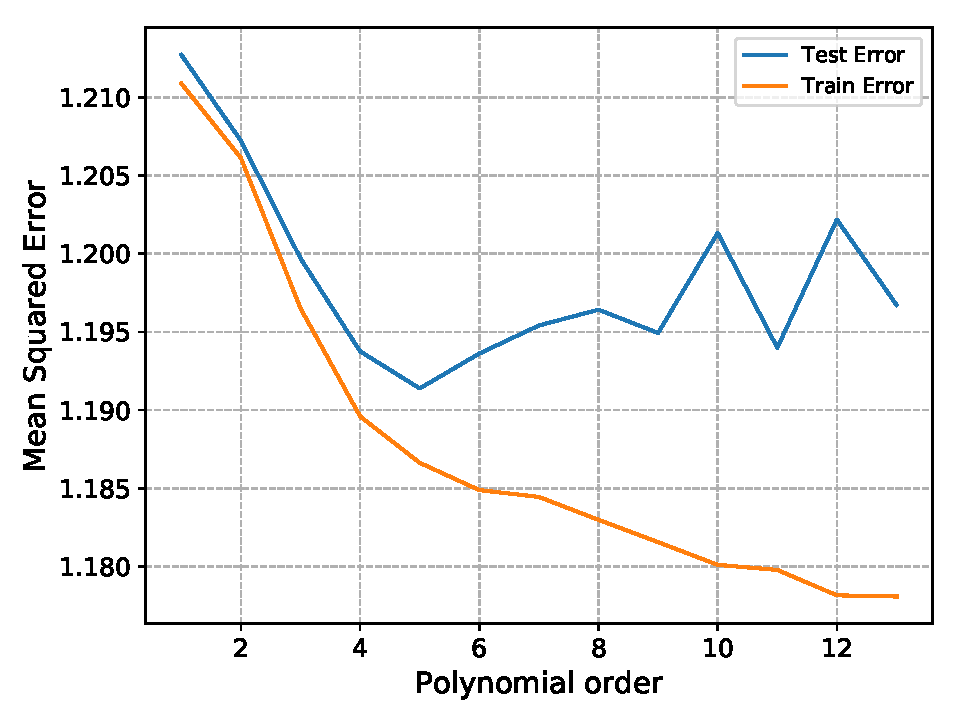
\includegraphics[scale=0.6]{c_OLSerr_train_test_vs_pdegree.pdf}
 	\caption{The training and test MSE for increasing model complexity, using Ordinary Least Squares and $k$-fold Cross Validation and the noisy dataset. While the test error reaches a minimum before increasing again, the training error will continuously decrease with increasing complexity.}
 	\label{fig:2}
 \end{figure}

If we instead calculate the MSE based on the real data, we get Figure \ref{fig:2a}. Here too we see that the 5th order polynomial fits the data the best.
 \begin{figure}[H]
	\centering
	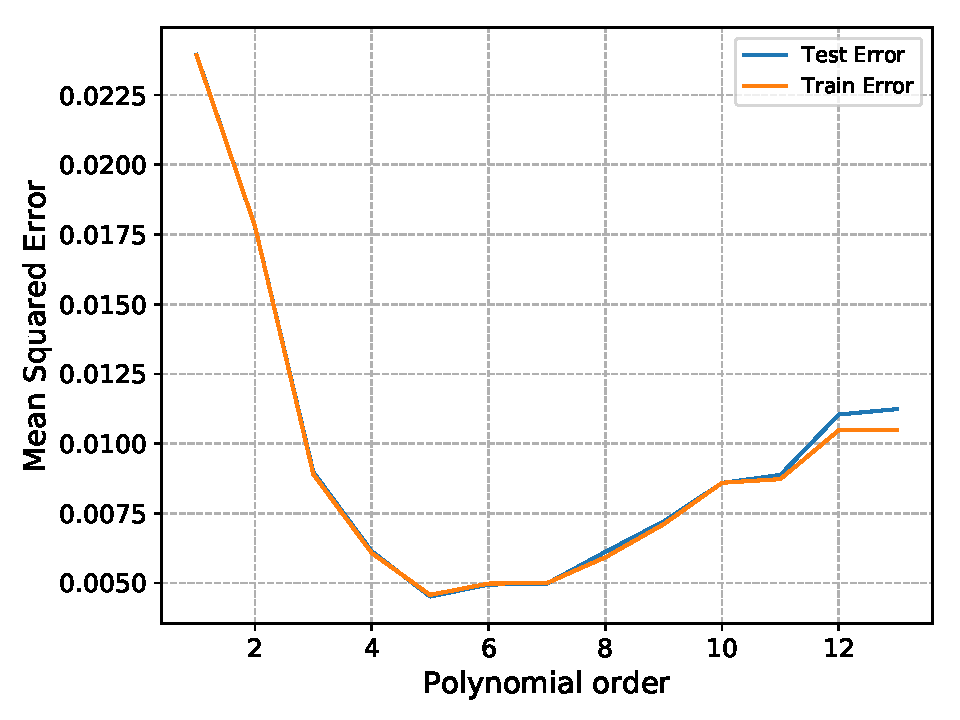
\includegraphics[scale=0.6]{c_OLSerr_train_test_vs_pdegree_no_noise.pdf}
	\caption{The training and test MSE for increasing model complexity, using Ordinary Least Squares and $k$-fold Cross Validation and the true dataset. While the test error reaches a minimum before increasing again, the training error will continuously decrease with increasing complexity.}
	\label{fig:2b}
\end{figure}
\subsubsection{Ridge regression analysis}
Now that we try a new method, we go back to starting with fitting a 5th order polynomial to the data. But here we must also take into account the penalization parameter $\lambda$ value. 

If we plot polynomial degrees against the MSE for various values of $\lambda$, we get the diagram in Figure \ref{fig:5}, and the close-up in Figure \ref{fig:6}. What we see is that a 5th order polynomial is favored for $\lambda=10^{-7} - 10^{-2}$, and the best fit value is $\lambda=10^{-2}$. However, we note that the difference in MSE is extremely small for $\lambda<10^{-2}$, making it uncertain which exact value of $\lambda$ is the best fit. We see this also in Figure \ref{fig:3}, where the Test error is quite noisy, and the best fit value becomes uncertain.

Nonetheless, we choose to continue on with a 5th order polynomial and $\lambda=1e-2$. The test and training error for this pair of variables can be seen in Figure \ref{fig:3}.

\begin{figure}[H]
	\centering
	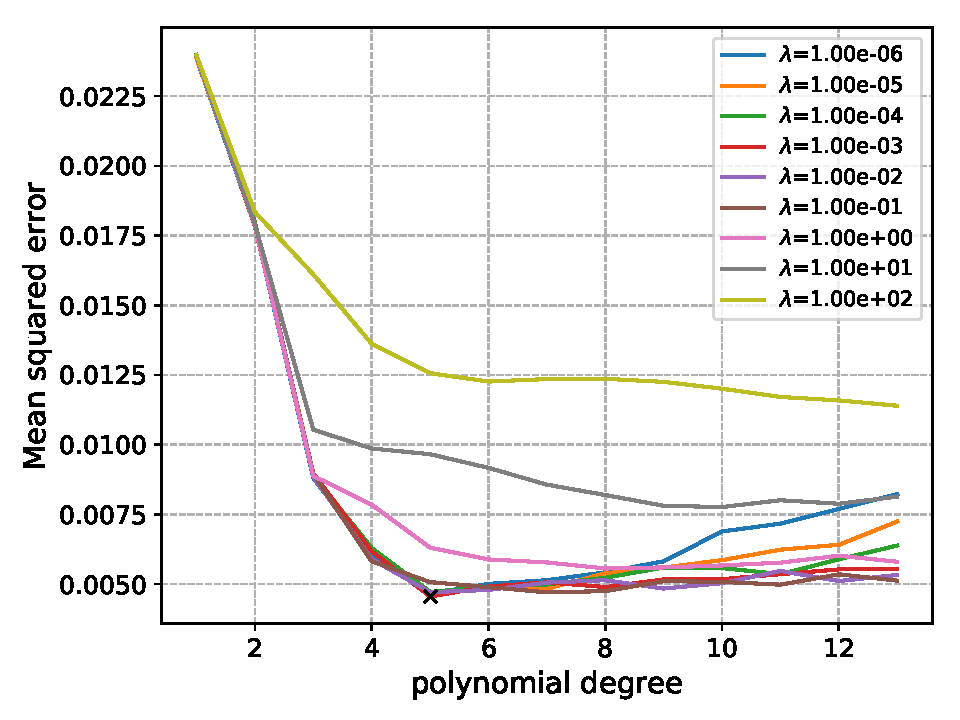
\includegraphics[scale=0.6]{d_Ridge_MSE_pdegree_lmbda.pdf}
	\caption{The MSE, calculated using the true model, for the test data for various $\lambda$ values and polynomial degrees, while using cross validation and Ridge regression. The minimum MSE value has been marked by a black $\times$.}
	\label{fig:5}
\end{figure}

\begin{figure}[H]
	\centering
	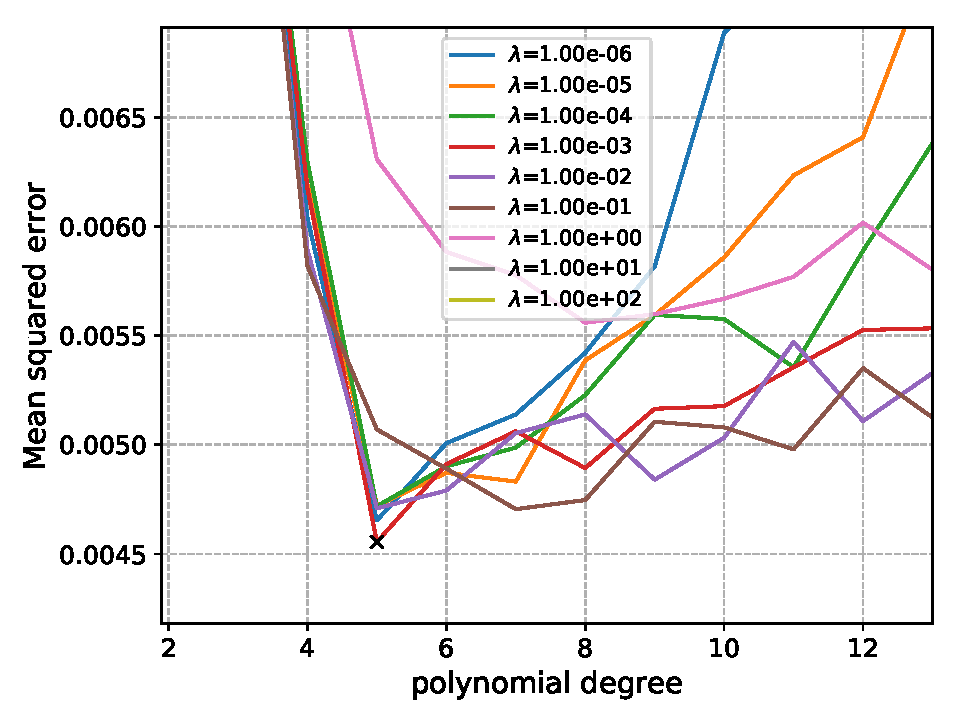
\includegraphics[scale=0.6]{d_Ridge_MSE_pdegree_lmbda_close.pdf}
	\caption{Close-up of the MSE, calculated using the true model, for the test and training data for various $\lambda$ values, while using cross validation and Ridge regression, for a fifth order polynomial. The minimum MSE value has been marked by a black $\times$.}
	\label{fig:6}
\end{figure}


 \begin{figure}[H]
	\centering
	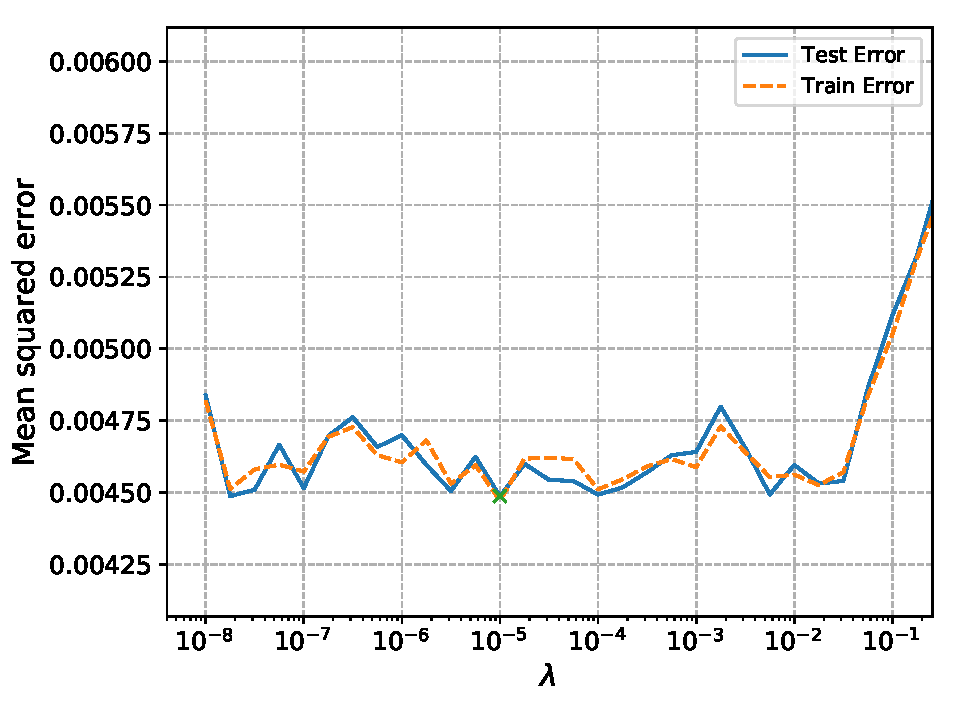
\includegraphics[scale=0.6]{d_lambda_vs_err_d5_close.pdf}
	\caption{The training and test error, calculated using the true model, for various $\lambda$ values, while using cross validation and a fifth order polynomial. The minimum MSE value has been marked by a yellow $\times$.}
	\label{fig:3}
\end{figure}

%The $\beta$-coefficients can be seen in Figure \ref{fig:Ridgebeta}
%\begin{figure}[H]
%	\centering
%	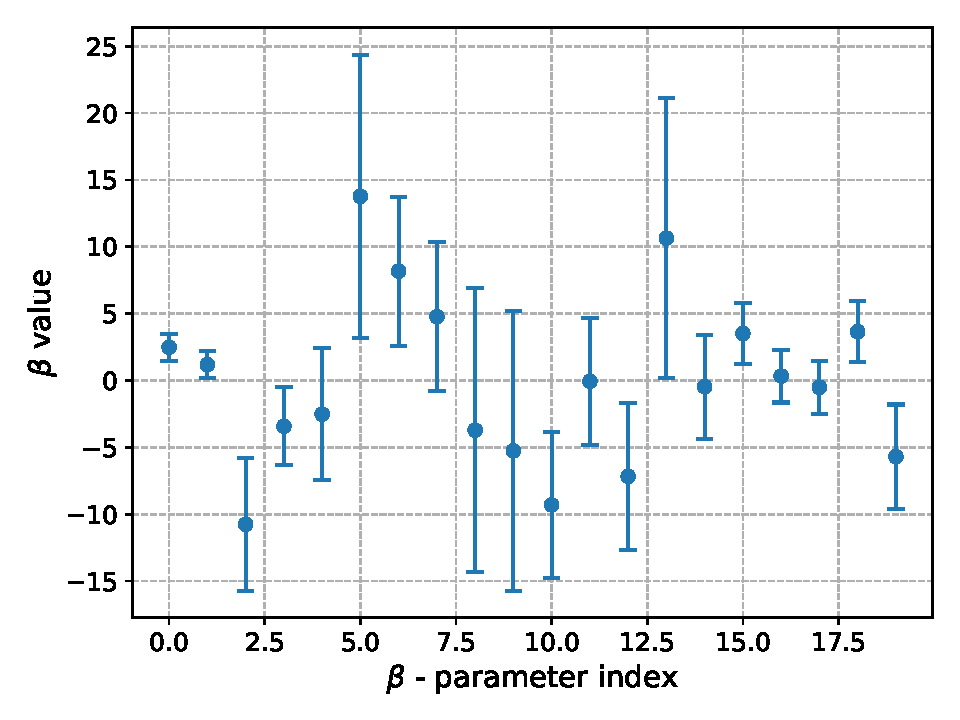
\includegraphics[scale=0.6]{d_CI_betaRidge_wb0.pdf}
%	\caption{The values of the parameters $\beta$ found from a Ridge regression analysis for a fifth order polynomial and $\lambda=10^{-3}$, are shown on the $y$-axis, while the index of the parameters are on the $x$-axis. The errorbars are calculated at 95\% confidence}
%	\label{fig:Ridgebeta}
%\end{figure}

%Without cross-validating, using a fifth order polynomial and $\lambda=10^{-3}$, the MSE score is $4.45\cdot10^{-3}$, and $R^2 = 0.95$.

\begin{figure}[H]
	\centering
	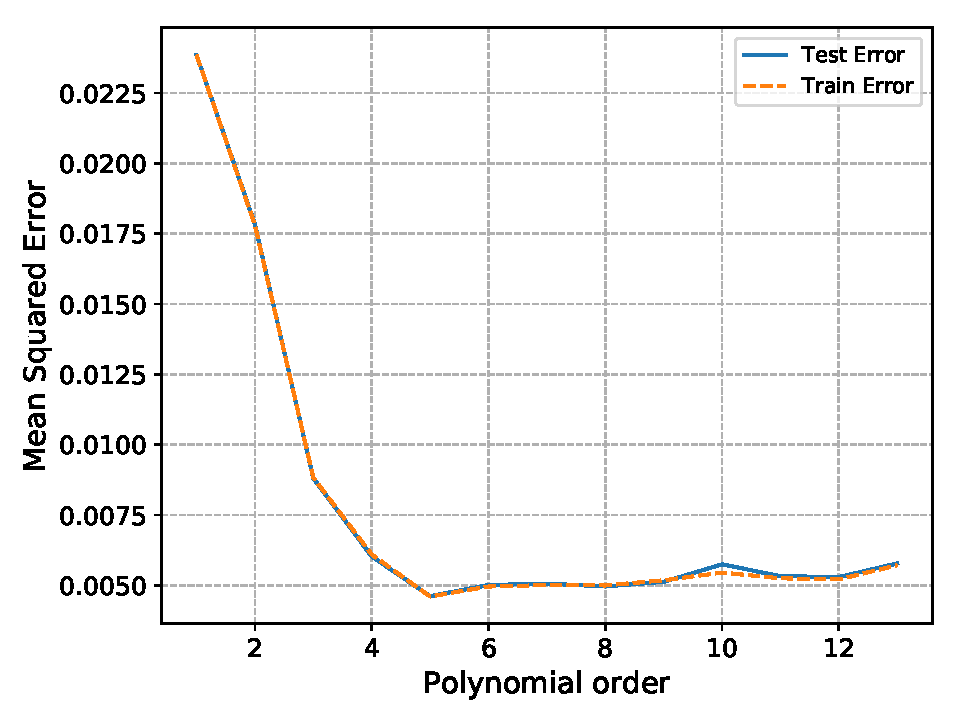
\includegraphics[scale=0.6]{d_Ridge_err_pdegree.pdf}
	\caption{The training and test MSE for increasing model complexity, using Ridge regression and $k$-fold Cross Validation. While the test error reaches a minimum before increasing again, the training error will continuously decrease with increasing complexity.}
	\label{fig:4}
\end{figure}


\subsubsection{Lasso regression analysis}
Finally, we use the Lasso method to find $\bm{{\tilde z}}$.
First we calcaulte the MSE as a function of polynomial order and $\lambda$. This can be seen in Figure \ref{fig:7}.

We again start from a 5th order polynomial, and find that, with cross-validation, $\lambda=2\cdot10^{-5}$ fit data best, as it had an predictive error at $MSE = 4.68\cdot 10^{-3}$ and $R^2=0.943$. For any lower $\lambda$ values, we get a warning that there is no converging. Having already standardized the data and increased the number of iterations and tolerance in \code{sklearn}'s \code{Lasso}, we elected not to test this further. This can be seen in Figure \ref{fig:8}. Here we find also that a 5th order polynomial fits the best, this time with $\lambda=10^{-5}$. We note that the increase in MSE is very small for increasing polynomial orders, for all $\lambda$. 

While running the calculations for $\lambda=10^{-6}$ and $\lambda=10^{-5}$ we did however get a no-convergence-warning.
Seeing as $\lambda=10^{-4}$ provides an almost as good fit, we will use that instead.

\begin{figure}[H]
	\centering
	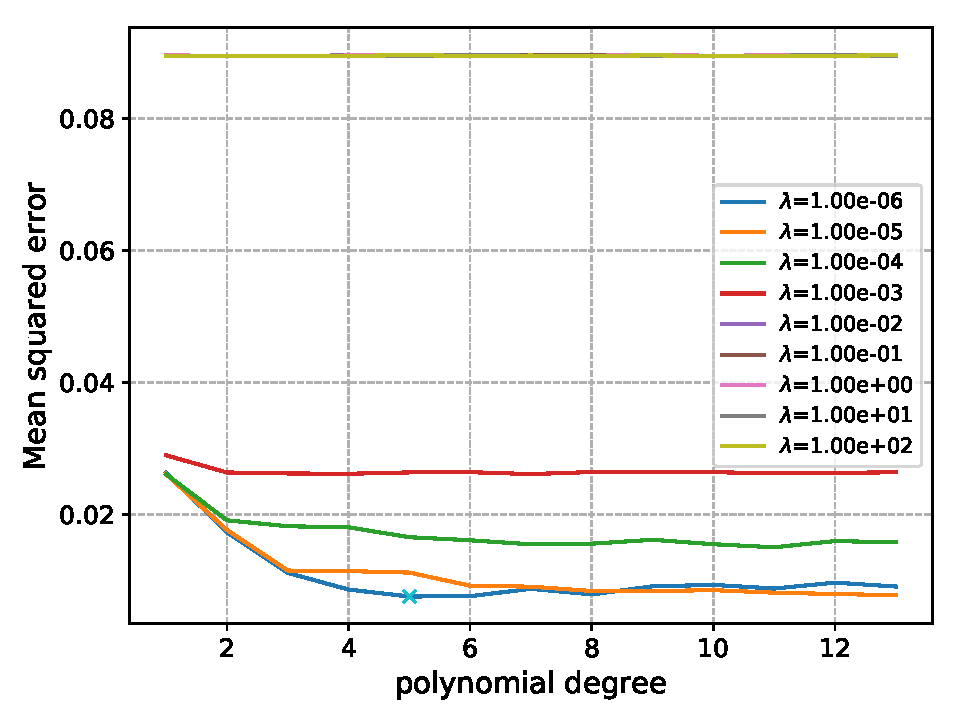
\includegraphics[scale=0.6]{e_Lasso_MSE_pdegree_lmbda.pdf}
	\caption{The MSE, calculated using the true model, for the test and training data for various $\lambda$ values, while using cross validation and Lasso regression, for a fifth order polynomial. The minimum MSE value has been marked by a blue $\times$.}
	\label{fig:7}
\end{figure}

\begin{figure}[H]
	\centering
	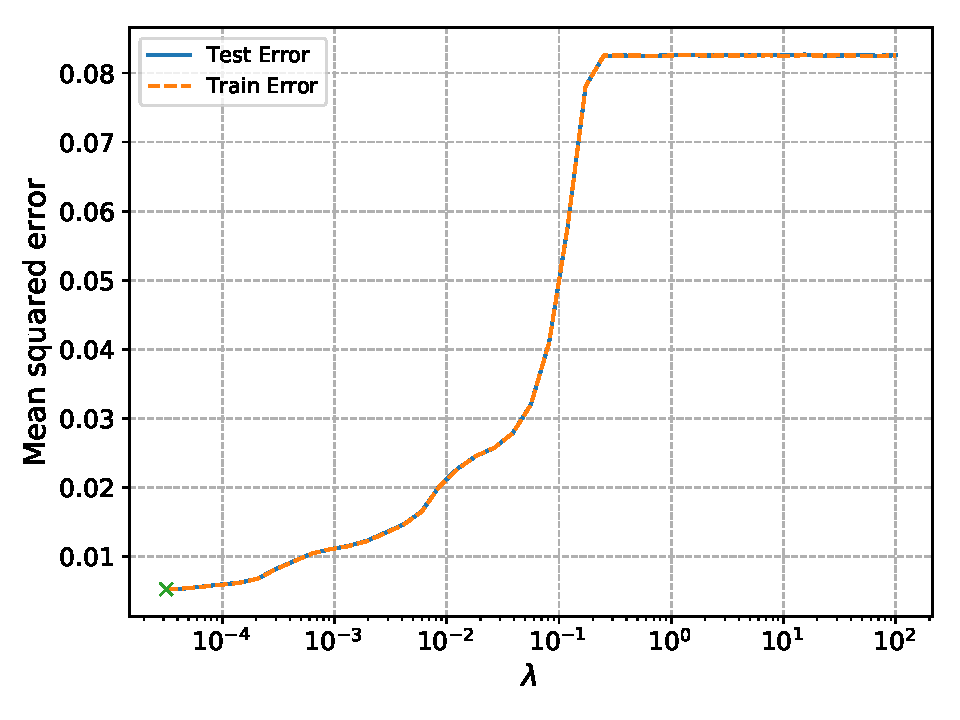
\includegraphics[scale=0.6]{e_lambda_vs_err_d5.pdf}
	\caption{The MSE, calculated using the true model, for the test data for various $\lambda$ values, while using cross validation and Lasso regression on a fifth order polynomial. The minimum MSE value has been marked by a yellow $\times$, although due to convergence issues, we will not use that one.}
	\label{fig:8}
\end{figure}


\subsection{Terrain analysis}
Here are the results from our linear regression analyses on data of a terrain in Norway. The original image, and the result of our chosen sampling, is seen in Figure \ref{fig:terrain}
\begin{figure}[H]
	\centering
	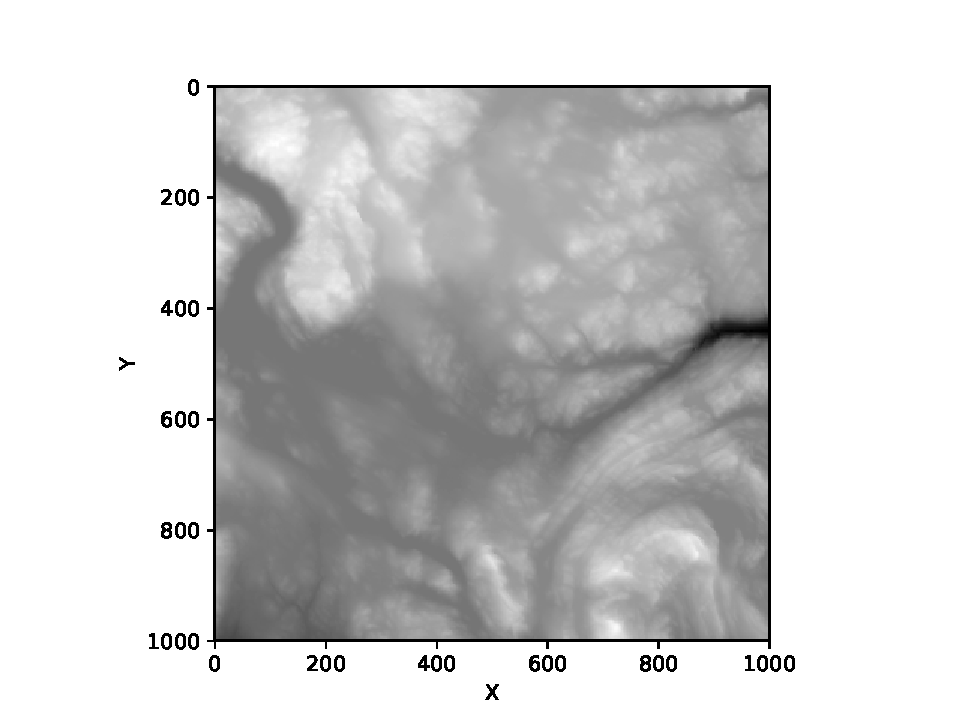
\includegraphics[scale=0.5]{terrain_cut.pdf}\hspace{-5em}
	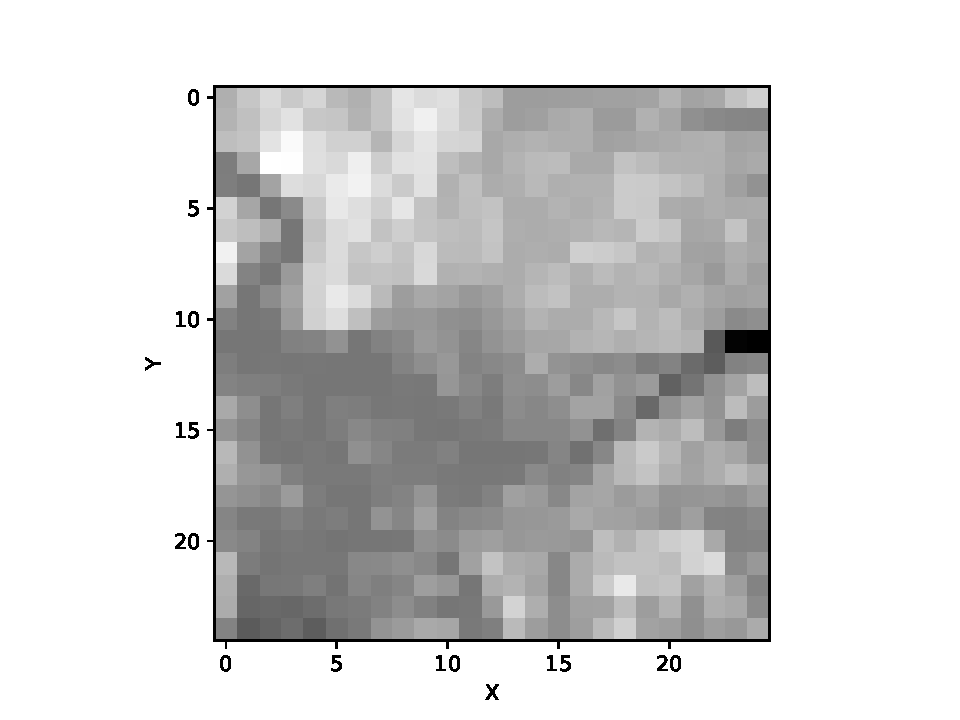
\includegraphics[scale=0.5]{terrain_cut_sample.pdf}
	\caption{To the left is the small cutout of the original data. To the right is the down-sampled image that we will work on.}
	\label{fig:terrain}
\end{figure}
Now, to find the best fit polynomial for an OLS, and also the best fit $\lambda$ for the Ridge and Lasso models, before we discuss which method fits the data the best.

The results of our analyses can be seen in Table \ref{tab:2}

We first performed an Ordinary Least Squares regression analysis, which included Cross-Validation. We did this for the training and testing set for various polynomial degrees. This can be seen in figure \ref{fig:7}.

We find that a 10th order polynomial minimizes the MSE test error the best, although this depends heavily on the amount of data we use. We found as expected, that the more data we used, the higher order polynomial was found to minimized MSE. In these cases, the test and training error were almost the same, meaning it is more difficult to overfit and start sampling the noise, but the higher the variance would become.

In the end the fit is a quite poor one, with $MSE=8413.40$, and  $R^2=0.609$. It is unclear why the MSE is so high, but we suspect there is something wrong with our calculations. However we obtained the same result using our own algorithm, and that by \code{sklearn}.
\begin{figure}[H]
	\centering
	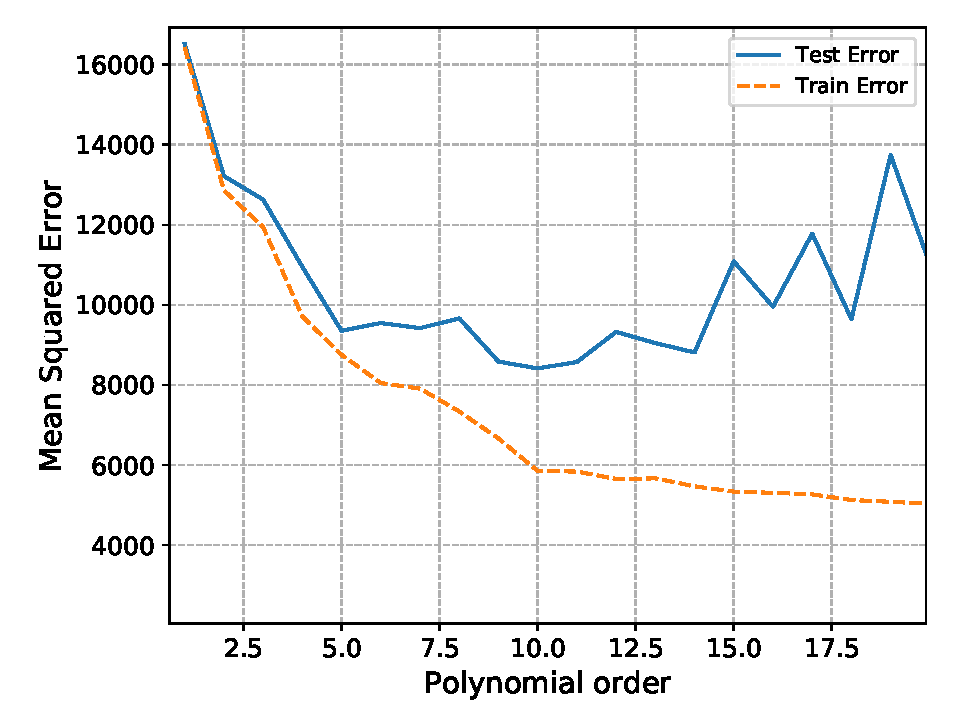
\includegraphics[scale=0.6]{g_OLS_err_pdegree_c1000s40.pdf}
	\caption{The testing and training error for various polynomial degrees, while using k-fold cross validation}
	\label{fig:10}
\end{figure}


\subsubsection{Ridge regression}
When performing a Ridge regression, we found again that a 10th order polynomial fit the data the best.

Fitting both $\lambda$ and the polynomial degree at the same time, we get the plot in figure \ref{fig:11}. We see that the curves are quite erratic, only the two highest $\lambda=1, 10^{-1}$ have a somewhat smooth descent before increasing again. This makes our estimate of both polynomial order and $\lambda$ uncertain. It seems that $\lambda=10^{-9}$ and $d=12$ might work as well, as the curve seem more "calm", but the MSE is slightly higher. 

%$MSE=8271.37$, and $R^2= 0.618$. All in all, a poor fit.

\begin{figure}[H]
	\centering
	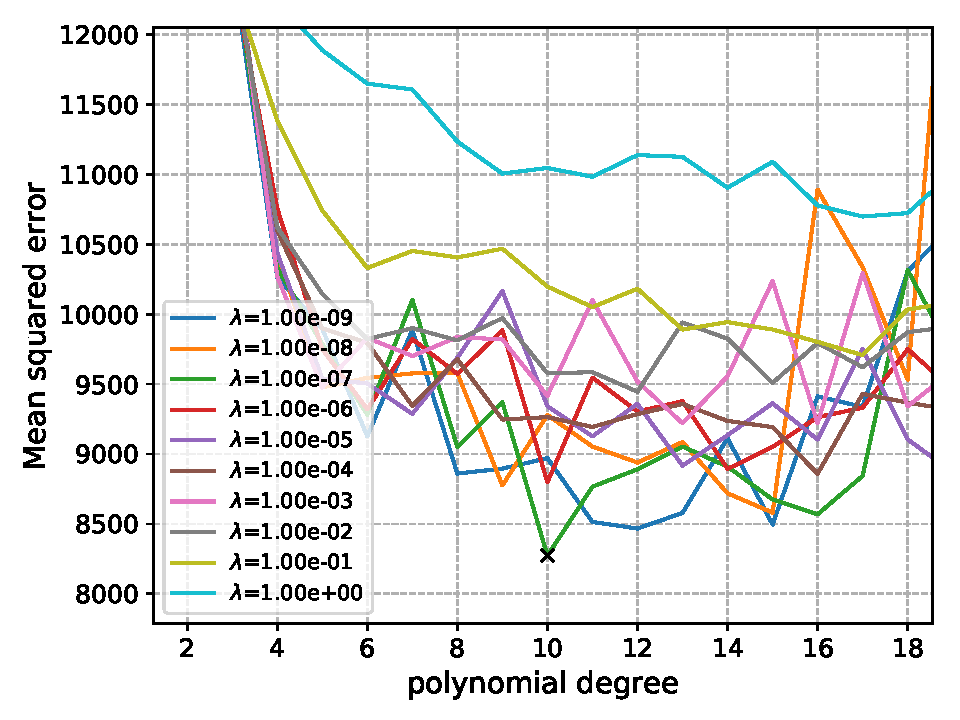
\includegraphics[scale=0.6]{g_Ridge_MSE_pdegree_lmbda.pdf}
	\caption{The Mean Square error calculated for various values of $\lambda$ and polynomial orders. The black $\times$ marks the best fit.}
	\label{fig:11}
\end{figure}

Like before, we plot the MSE against $\lambda$ for the polynomial we found that reduced the MSE the most. The test error seems quite erratic, and there is no minimum, as the training and test error is increasing. Can be due to overfitting for the test error, but what it means for the training data, we are not certain. It flattens out at very small $\lambda$, meaning an OLS will propbably fit better.
\begin{figure}[H]
	\centering
	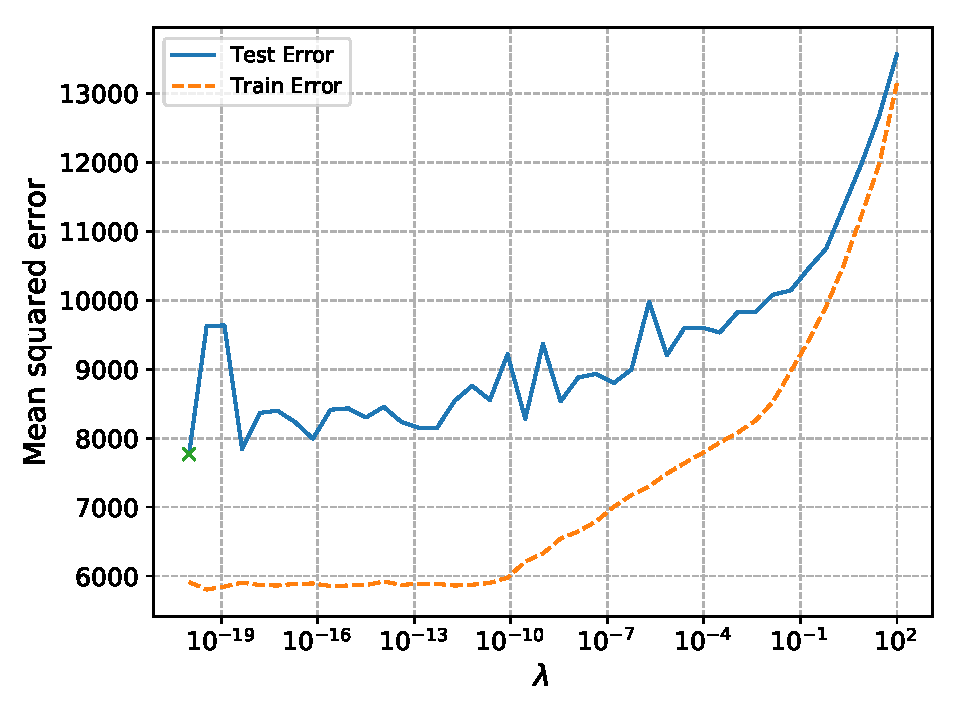
\includegraphics[scale=0.6]{g_Ridge_lambda_vs_err_d10.pdf}
	\caption{The MSE, calculated for various $\lambda$ values, while using cross validation and Ridge regression on a 10th order polynomial. The minimum MSE value has been marked by a yellow $\times$}
	\label{fig:12}
\end{figure}

\subsubsection{Lasso}
We have a hard time performing the Lasso regression analysis. The computations take a very long time, and the small $\lambda$ that seems to be favored, throw out a no-convergence warning.
We therefore assume that a 10th order polynomial is still the best option, and calculate the MSE for various $\lambda$, as seen in Figure \ref{fig:13}. Here too, the curve is erratic, and there is no well-defined minimum.
\begin{figure}[H]
	\centering
	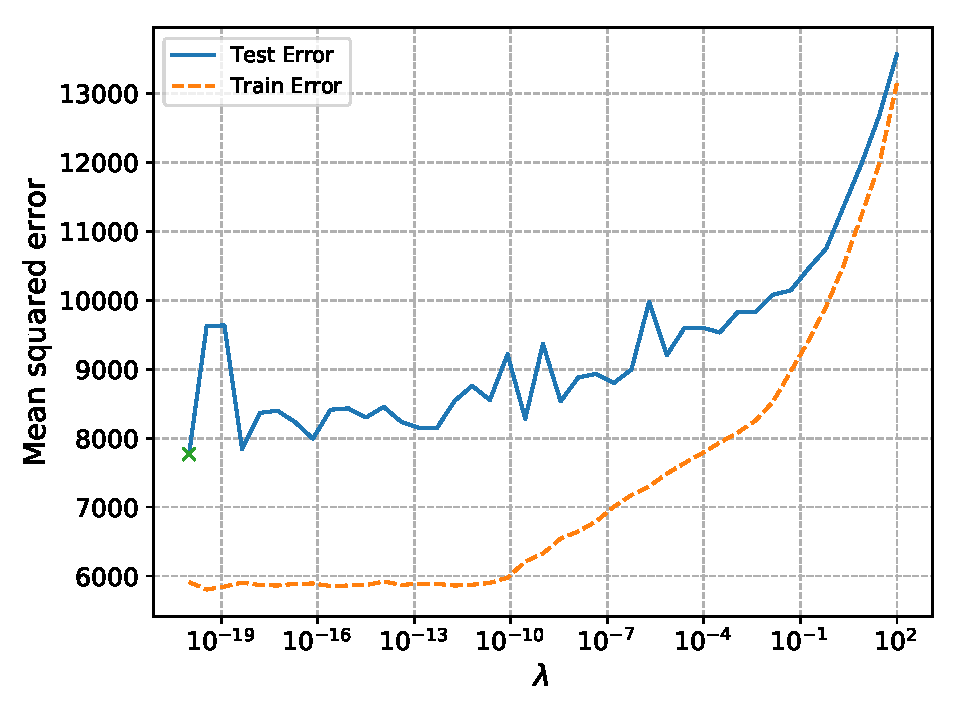
\includegraphics[scale=0.6]{g_Ridge_lambda_vs_err_d10.pdf}
	\caption{The MSE, calculated for various $\lambda$ values, while using cross validation and Lasso regression on a 10th order polynomial. The minimum MSE value has been marked by a yellow $\times$}
	\label{fig:13}
\end{figure}
min error: 8333.226101945776
min error poly: 29
max r2 score: 0.6207354507501407

Need a higher polynomial

\section{Discussion}\label{sec:discussion}
For our data generated from the Franke function, we find that, irregardless of method, a 5th order polynomial fits our data the best. The $\beta$-coefficients, do however, have very large confidence intervals.

The $MSE$ increases slightly as we change from OLS to Ridge and to Lasso, but only at the fourth decimal spot. Similarly, the $R$ score does not really change, staying at approximately $R^2=0.95$ This makes it difficult to say if one method is more appropriate than another.
In Table\ref{tab:1} The $R^2$ and $\mathrm{MSE}$ scores are shown for the best fit models. We can see from this, that the OLS method wins out by a small margin.
\begin{table*}[t]
	\centering
	\begin{threeparttable}
		\centering
		\caption{The $R^2$ and $MSE$ scores for the OLS, Ridge, and Lasso regression for the best fitted polynomials, $d$ and $\lambda$.}
		\label{tab:1}
		\begin{tabular}{ccccc}
			\toprule\toprule
			Model & $d$ & $\lambda$ & MSE & $R^2$\\
			\midrule
			OLS			& 5 	& - 	&$4.62\cdot10^{-3}$ & 0.944\\
			Ridge		& 5 	& $10^{-2}$ &$4.71\cdot10^{-3}$ &0.943 \\
			Lasso		& 5 	&$10^{-4}$ & $ 5.24\cdot10^{-3}$ &0.936\\
			\bottomrule\bottomrule
		\end{tabular}
	\end{threeparttable}
\end{table*}

Initially, we had fewer points, but this proved to make our analyses difficult, as the noise was of the same order as the Franke Function, making it hard to sample the true function. Our MSE was then approximately 0.02, and $R^2$ lied around $\pm0.1$. 
We found that this could be remedied by lowering the noise, by, for instance lowering its standard deviation, or by increasing the amount of data points. We chose the latter. We suspect there may be something wrong in the way the confidence intervals of the $\beta$ parameters are calculated, as they are very large at certain data points, but we are not able to find it.

Performing an analysis on the terrain data proved difficult. The minimum MSE and corresponding $R^2$-scores can be seen in Table \ref{tab:2}. It would seem that the Lasso managed to recreate the terrain the best, but this does not say much, as they all have an $R^2\approx0.6$, and the $\lambda$-values being as uncertain as they are.

\begin{table*}[t]
	\centering
	\begin{threeparttable}
		\centering
		\caption{The $R^2$ and $MSE$ scores for the OLS, Ridge, and Lasso regression for the best fitted polynomials, $d$ and $\lambda$.}
		\label{tab:2}
		\begin{tabular}{ccccc}
			\toprule\toprule
			Model & $d$ & $\lambda$ & MSE & $R^2$\\
			\midrule
			OLS			& 10 	& - 	&$8413.40$ & 0.609\\
			Ridge		& 10 	& $10^{-7}$ &$8271.37$ &0.618 \\
			Lasso		& 10 	& - & $7998.89$ &$0.628$ \\
			\bottomrule\bottomrule
		\end{tabular}
	\end{threeparttable}
\end{table*}

As for the reason for this, we are not certain. I suspect that if, instead of just skipping over pixels, we calculated the median, or average of neighboring pixels, applyed a Gaussian blur, then the data to fit would have been smoother, and our regression methods might have had it easier estimating a good $\bm{\tilde y}}$. 
We initially tried to do this, but time ran short near the end. The challenge then is not undersampling the original terrain image to much so that it was still recognizable, but not oversampling it either, so that wedo not get a high variance, very higher order polynomial.

Personal note at the end. I found this project somewhat confusing at times. It seemed that different instructors would endorse, or emphasize certain things quite differently. The foremost example being whether or not to penalize the intercept, where there were quite conflicting replies on piazza. Beyond that, I am aware that this report could have been more filled in in places, but I have done the best with the time I had.
 
\section{Conclusion}\label{sec:conclussion}
In this project we have used three different linear regression models: The Ordinary Least Squares, Ridge regression, and Lasso regression. 

We first created noisy data from the known Franke function, that we used to  train our algorithm, and make a prediction as to the true function $f$. We then calculated the Mean Square Error(MSE) and $R^2$ score to find the model and the parameters that minimized the MSE. We concluded that the OLS recreated the true underlying function the best, with an $MSE=4.62\cdot10^{-3}$ and $0.944$.

We performed also linear regression on data taken of a terrain in Norway. We scaled down the image simply by skipping over pixels, and then tried to model the image. In this case, we found that all three models made very poor predictions, where $R^2\approx0.6$, and a very high $MSE\sim 10^3$. The reason for the high MSE was not clear, most likely there is a mistake somwhere in our algorithm. In the future, to improve the fit, we could instead, or in addition to, skipping pixels, blur the image with a Gaussian filter.

\bibliography{library}

\end{document}